%%%%%%%%%%%%%%%%%%%%%%%%%%%%%%%%%%%%%%%%%
% Short Sectioned Assignment
% LaTeX Template
% Version 1.0 (5/5/12)
%
% This template has been downloaded from:
% http://www.LaTeXTemplates.com
%
% Original author:
% Frits Wenneker (http://www.howtotex.com)
%
% License:
% CC BY-NC-SA 3.0 (http://creativecommons.org/licenses/by-nc-sa/3.0/)
%
%%%%%%%%%%%%%%%%%%%%%%%%%%%%%%%%%%%%%%%%%

%----------------------------------------------------------------------------------------
%	PACKAGES AND OTHER DOCUMENT CONFIGURATIONS
%----------------------------------------------------------------------------------------

\documentclass[paper=a4, fontsize=11pt]{scrartcl} % A4 paper and 11pt font size

\usepackage[T1]{fontenc} % Use 8-bit encoding that has 256 glyphs
\usepackage{fourier} % Use the Adobe Utopia font for the document - comment this line to return to the LaTeX default
\usepackage[english]{babel} % English language/hyphenation
\usepackage{amsmath,amsfonts,amsthm} % Math packages

\usepackage{lipsum} % Used for inserting dummy 'Lorem ipsum' text into the template

\usepackage{sectsty} % Allows customizing section commands
\allsectionsfont{\centering \normalfont\scshape} % Make all sections centered, the default font and small caps

\usepackage{fancyhdr} % Custom headers and footers
\pagestyle{fancyplain} % Makes all pages in the document conform to the custom headers and footers
\fancyhead{} % No page header - if you want one, create it in the same way as the footers below
\fancyfoot[L]{} % Empty left footer
\fancyfoot[C]{} % Empty center footer
\fancyfoot[R]{\thepage} % Page numbering for right footer
\renewcommand{\headrulewidth}{0pt} % Remove header underlines
\renewcommand{\footrulewidth}{0pt} % Remove footer underlines
\setlength{\headheight}{13.6pt} % Customize the height of the header

\numberwithin{equation}{section} % Number equations within sections (i.e. 1.1, 1.2, 2.1, 2.2 instead of 1, 2, 3, 4)
\numberwithin{figure}{section} % Number figures within sections (i.e. 1.1, 1.2, 2.1, 2.2 instead of 1, 2, 3, 4)
\numberwithin{table}{section} % Number tables within sections (i.e. 1.1, 1.2, 2.1, 2.2 instead of 1, 2, 3, 4)

\setlength\parindent{0pt} % Removes all indentation from paragraphs - comment this line for an assignment with lots of text

\usepackage{graphicx}
\graphicspath{ {./img/} }
\usepackage{float}

%----------------------------------------------------------------------------------------
%	TITLE SECTION
%----------------------------------------------------------------------------------------

\newcommand{\horrule}[1]{\rule{\linewidth}{#1}} % Create horizontal rule command with 1 argument of height

\title{	
\normalfont \normalsize 
\textsc{Department of Computer Science, University of Helsinki} \\ [25pt] % Your university, school and/or department name(s)
\horrule{0.5pt} \\[0.4cm] % Thin top horizontal rule
\huge Unsupervised Machine Learning \newline Exercise1: Principle Component Analysis \\ % The assignment title
\horrule{2pt} \\[0.5cm] % Thick bottom horizontal rule
}

\author{Han Xiao(014343753)} % Your name

\date{\normalsize\today} % Today's date or a custom date

\begin{document}

\maketitle % Print the title

%----------------------------------------------------------------------------------------
%	PROBLEM 1
%----------------------------------------------------------------------------------------

\section{Question 1}

Taking some time of tweaking the means and covariance matrices, the final scatter plots for 4 data sets are as follows:

\begin{figure}[H]
  \centering
  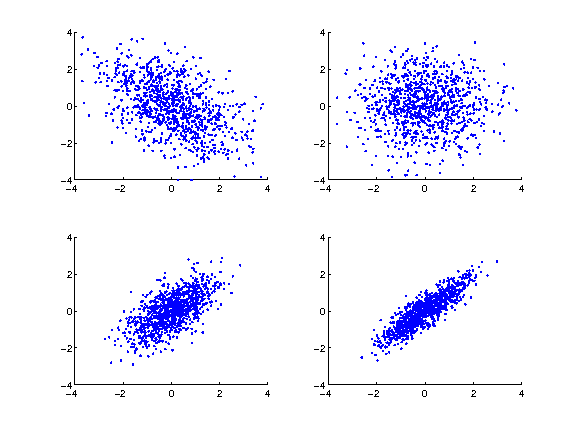
\includegraphics[scale=.7]{scatter_points}
  \caption{Approximated scatter plots for the given 4 data sets}
\end{figure}


%------------------------------------------------


%----------------------------------------------------------------------------------------
%	PROBLEM 2
%----------------------------------------------------------------------------------------

\section{Question 2}
The process to do PCA on data of any dimension is basically as follows:

\begin {enumerate}
\item compute the covariance matrix of the data, $C$
\item do eigenvalue decomposition on the $C$ and return the eigen values as $D$ and eigen vectors as $U$(the same notation as the lecture notes)
\end {enumerate}

  
%----------------------------------------------------------------------------------------
%	PROBLEM 3
%----------------------------------------------------------------------------------------

\section {Question 3}

I plotted  directions for both PCs for all of the 4 data sets, the plot is as followed, in which red lines denote the PC directions.

\begin{figure}[H]
  \centering
  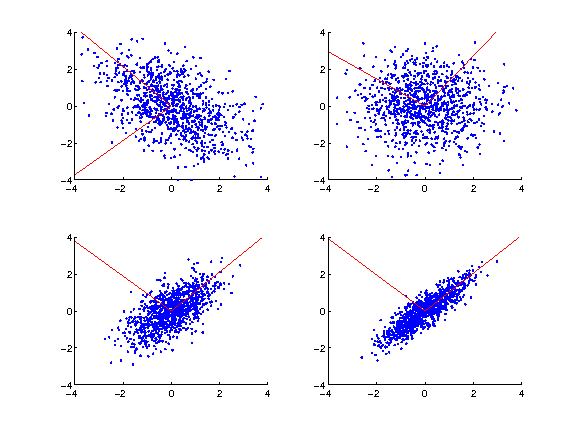
\includegraphics[scale=.7]{eigen_vectors}
  \caption{Directions of principal components for all above data sets}
\end{figure}


%----------------------------------------------------------------------------------------
%	PROBLEM 4
%----------------------------------------------------------------------------------------

\section {Question 4}

I projected the first data set on both PC directions and the variance for each direction are 0.9606 and 3.0424 respectively, which corresponds to the eigenvalue exactly.

This makes a lot of sense as the intuition of the computed eigenvalues are the variances explained by the corresponding eigen vectors. 

\begin{figure}[H]
  \centering
  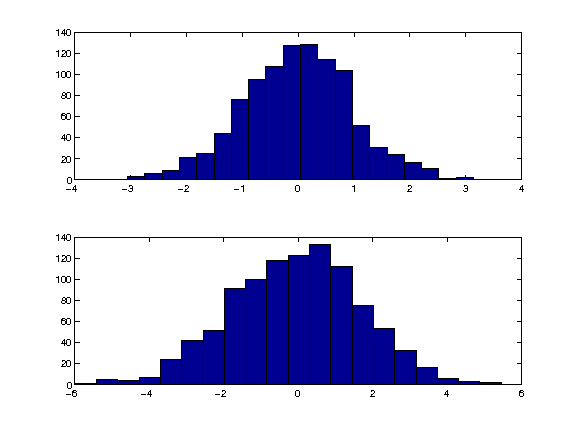
\includegraphics[scale=.7]{histogram}
  \caption{Histograms of the projected values on each PC direction}
\end{figure}

%----------------------------------------------------------------------------------------
%	PROBLEM 5
%----------------------------------------------------------------------------------------

\section {Question 5}

The scatter plot of artificial data is given below, which resembles the first data set quite a lot. After performing the eigenvalue decomposition of the covariance matrix, the eigenvalues and eigen vectors are $[1.0009, 3.2130]$ and  $[-0.7324, -0.6809; -0.6809, 0.7324]$, which are very close to the given vectors($v_1$ and $v_2$) and the variance respectively.

This result makes a lot of sense as the process of creating the artificial data is like the reconstruction process.

\begin{figure}[H]
  \centering
  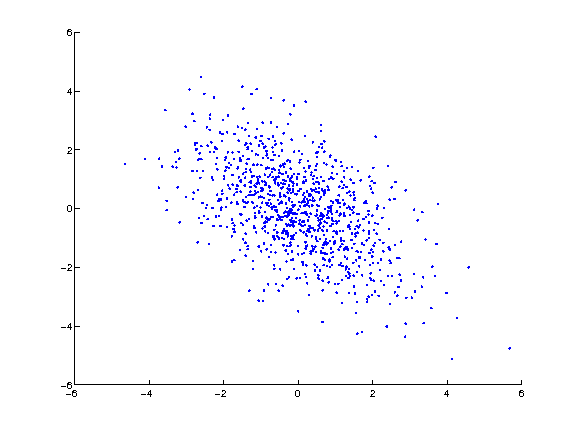
\includegraphics[scale=.7]{artificial_data}
  \caption{Artificially created data according to the specification in Question 5}
\end{figure}

%----------------------------------------------------------------------------------------
%	PROBLEM 6
%----------------------------------------------------------------------------------------

\section {Question 6}

\begin{figure}[H]
  \centering
  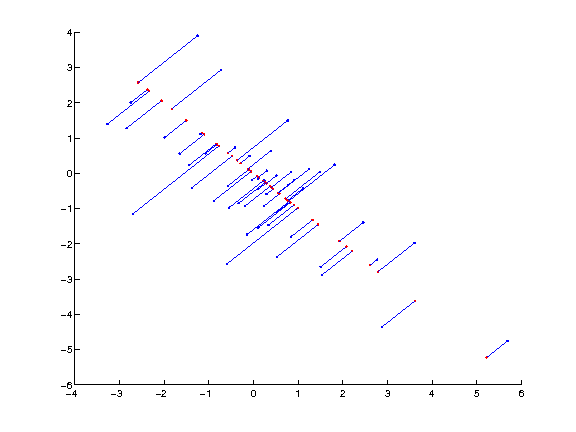
\includegraphics[scale=.7]{reconstruction}
  \caption{Reconstructed data in terms of the second PC direction}
\end{figure}

In case when the reconstruction error is minimized, the second eigen vector, $v_2$ is used and the average reconstruction error is 1.0030, which is the part of variance (which is 1) that can be explained by $v_1$. However, as we use only $v_2$, this part of variance is not explained and thus is incorporated into the error.

To gain more intuition, reconstruction using $v_1$ gives an average reconstruction error 3.2069, which corresponds the variance explained by $v_2$.
%----------------------------------------------------------------------------------------

\end{document}
